\section{Work Profiling}

In this section, we describe how to measure work online. Total work is just the sum of the costs of all executed basic blocks, so it is
possible to embed its computation into the execution of the program. A naive instrumentation would use a global counter initialized at the
interception value, $\varepsilon$. Each basic block would then have only to increment this counter with the total cost of its instructions
every time it is executed. Although easy to implement, the naive approach introduces a significant overhead.

Previous work on basic block profiling has proposed optimal ways for instrumenting the code with as little overhead as possible without
losing any profiling information~\citep{knuth73,ball94}. The underlying idea is to instrument only a subset of the basic blocks of a
function and use the function's CFG to calculate execution counts for the rest. We can use the same idea for our purposes. Work profiling
and basic block profiling are similar, both need to count how many times each basic block was executed. The only important difference is
that we do not have to store the execution count of each basic block, only the total work. 

Graph theory shows that we can calculate precisely the frequencies of all edges between basic blocks if we choose a spanning tree of the
function CFG and instrument the edges not in the tree. To make the instrumentation probe placement optimal, we choose the maximum spanning
tree, with the edge weights representing edge frequency estimates. As many high frequency edges as possible will be in the maximum spanning
tree and they will not be instrumented. 

\begin{figure}[t]
\centering {
  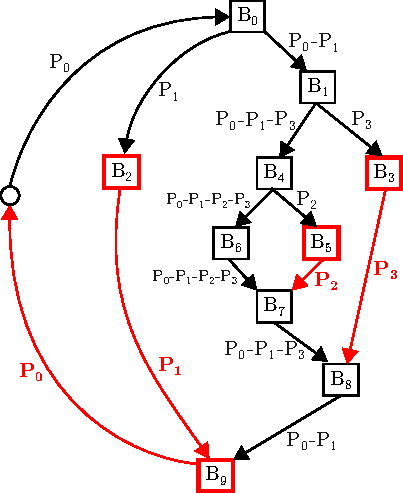
\includegraphics[scale=0.75]{figs/cfg-example.pdf}\\\vspace{1ex}
  \resizebox{0.45\textwidth}{!}{
  %\scalebox{0.8}{
     \begin{minipage}{0.5\textwidth}
     Instrumented value for each probe $P_i$:
     \begin{align*}
     \omega(P_0) &= w(B_0) + w(B_1) + w(B_4) + w(B_6) + w(B_7) + w(B_8) + w(B_9)\\
     \omega(P_1) &= w(B_2) - w(B_1) - w(B_4) - w(B_6) - w(B_7) - w(B_8)\\
     \omega(P_2) &= w(B_5) - w(B_6)\\
     \omega(P_3) &= w(B_3) - w(B_4) - w(B_6) - w(B_7)
     \end{align*}
     \end{minipage}
  }
}
  \caption{Example of a CFG with its maximum spanning tree in black. Basic blocks and edges highlighted in red are instrumented.
    Instrumenting them is enough for calculating the total work performed by the whole CFG.}
  \label{fig:cfg-example}
\end{figure}

In contrast to the naive instrumentation where each basic block records only its own amount of work, with the optimal profiling the work
counter increments needs to take other basic blocks into account. Figure~\ref{fig:cfg-example} shows an example CFG, where the instrumented
blocks are marked with red. In this example, executing block $B_3$ implies also executing $B_1$ and not executing $B_4$. We compute the
aggregated value of work for each probe in two steps: \textit{(i.)} we propagate information about the probes through the edges of the CFG,
as symbolic expressions, and then \textit{(ii.)} we use these edge flows to compose the aggregated value of the probes.

The symbolic expressions in the edges can then be used to compose the aggregated
value of the probes.
These symbolic expressions describe the probes that are in the same path of the
edge (positive terms) and those that are in complementary paths (negative
terms).
Therefore, the positive terms in the summed symbolic expression of a
basic block indicate that the amount of work of this basic block will be
incremented in the probes represented by these positive terms.
Similarly, the negative terms indicate that the amount of work of this basic block
will be decremented in the probes represented by these negative terms.
For example, because the symbolic expression for the basic block $B_8$ is $P_0 - P_1$,
the amount of work of $B_8$, denoted by $w(B_8)$, is incremented in probe $P_0$
and decremented in $P_1$.

\paragraph{Populating the edge flows:}
Intuitively, if all the edge flows are known for the complement of a spanning tree
then at any leaf of the spanning tree there is only one unknown edge flow.
This unknown edge flow can be calculated by Kirchhoff's first law.
This process repeats as a bottom-up propagation until all the unknown edge flows
have been calculated.
This algorithm can be formally defined as a post-order traversal on the spanning
tree.
Let $G$ be the CFG.
This algorithm first initializes the edge flows $D_{(u,v)}$, for each edge
$(u,v)$ in the CFG, as follows:
\[
D_{(u,v)} \gets
\begin{cases}
    P_{(u,v)} & \quad \text{if edge $(u,v)$ has a probe $P_{(u,v)}$}\\
    0       & \quad \text{otherwise}
\end{cases}
\]
Afterwards, for each vertex $u\in G$, in a post-order traversal of the spanning tree,
we can use the Kirchhoff's first law and apply the following operations
in a symbolic fashion:
\[
\Sigma^+_u = \sum_{v\in N^+(u)} D_{(u,v)}
\]
\[
\Sigma^-_u = \sum_{v\in N^-(u)} D_{(v,u)}
\]
\[
\forall v\in N^+(u):  D_{(u,v)} \gets
\begin{cases}
    D_{(u,v)} & \quad \text{if $D_{(u,v)}\neq 0$}\\
    \Sigma^-_u - \Sigma^+_u       & \quad \text{otherwise}
\end{cases}
\]
\[
\forall v\in N^-(u):  D_{(v,u)} \gets
\begin{cases}
    D_{(v,u)} & \quad \text{if $D_{(v,u)}\neq 0$}\\
    \Sigma^+_u - \Sigma^-_u       & \quad \text{otherwise}
\end{cases}
\]

\paragraph{Composing the aggregated value of the probes:}
If $x$ is a symbolic expression, then $\kappa_P(x)$ represents the coefficient
of the term $P$ in $x$.
In our case, $\kappa_P(x)$ will belong to the set $\{-1,0,1\}$.
Then, for all probes $P$:
\[
\omega(P) = \sum_{u\in G} \kappa_P(\Sigma^+_u)w(u)
\]

\subsection{Relaxed Instrumentation}

Although the optimal instrumentation significantly reduces the profiling
overhead when compared to the naive instrumentation, from an average overhead
of 79\% to 13\%, in some critical cases, even the optimal instrumentation can
result in overheads of up to 60\% (see benchmark \texttt{adpcm\_d} in Figure~\ref{fig:overhead-O3}).
In order to further reduce the overhead in these critical cases, we propose a
relaxation strategy that offers a trade-off between accuracy and overhead.
While the optimal instrumentation places probes in edges that are
less likely to be executed, the relaxation removes probes that are
more likely to be executed but add little to the final work metric.

% \begin{figure}[h]
%   \centering
%   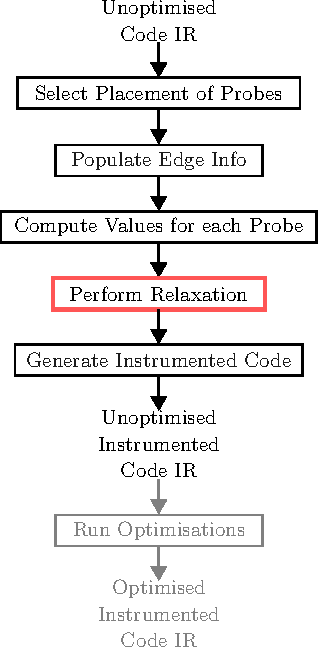
\includegraphics[scale=0.85]{figs/relax-instr-diagram.pdf}
%   \caption{Overview of the work instrumentation algorithm, including the relaxation technique.}
%   \label{fig:relax-instr-diagram}
% \end{figure}

%Figure~\ref{fig:relax-instr-diagram} shows an overview of the relaxed instrumentation algorithm.
%The highlighted step is introduced by the relaxed instrumentation on top of the previously defined optimal profiling.
The relaxation strategy performs a post processing on the resulting instrumentation of the optimal algorithm.
This post processing identifies probes that add little to the work metric, and removes their instrumentation.
In order to guarantee an upper bound for the dynamic error in the profiling measurement,
the relaxation algorithm applies a constrained post-processing on a per DAG (directed acyclic graph) basis.
By constraining the relaxation within each DAG by a maximum allowed static error,
it guarantees that the overall relaxation will also be constrained by the same bound.

The relaxation starts by extracting DAGs from the CFG.
First, the algorithm extracts all the subgraphs that represent a loop or the outer most region of the function.
Afterwards, these subgraphs are transformed into DAGs by ignoring the backedge
and also by considering that any loop within the subgraph is never executed,
i.e., only the headers of the inner loops are actually included into the DAG.
Figure~\ref{fig:cfg-relax-example} shows a CFG partitioned into two DAGs (consider
only basic blocks and edges completely inside the yellow and green boundaries).

\begin{figure}[t]
  \centering
  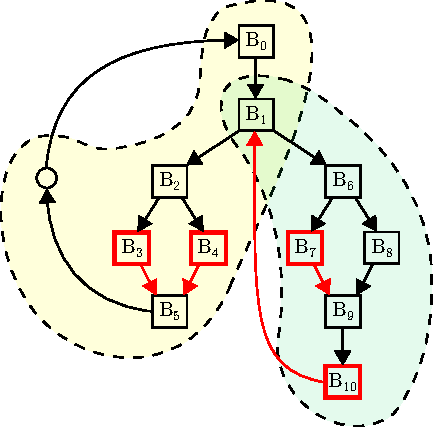
\includegraphics[scale=0.75]{figs/cfg-relax-example.pdf}
  \caption{Example of a CFG containing a loop and its decomposition into DAGs.
           The DAGs are the subgraphs within the dashed boundaries.}
  \label{fig:cfg-relax-example}
\end{figure}

%\begin{lstlisting}[caption={Optimal placement of probes for block frequency.}, label={lst:instrumentCFG}]
%// Input: CFG
%relaxInstrumentation(G) {
%  for loop in G:
%     DAG = colapseInnerLoops(loop)
%     relaxInstrumentedDAG(DAG)
%  DAG = colapseInnerLoops(G)
%  relaxInstrumentedDAG(DAG)
%}
%\end{lstlisting}

For every DAG with a set of probes $\{P_0, P_1, \ldots, P_k\}$,
we select a subset of the probes to be removed, subject to
the maximum allowed percentage error, $M$.
This strategy can be modeled as a 0-1 Knapsack problem:
\begin{gather*}
\textrm{max.}\quad\sum_{i=0}^{k} f(P_i)x_i,\quad
\textrm{s.t.}\quad\sum_{i=0}^{k} \varepsilon(P_i)x_i \leq M \\
x_i\in\{0,1\}, i\in\{0,\ldots,k\}
\end{gather*}
where $f(P_i)$ is the execution frequency of probe $P_i$, $x_i$ denotes the
probes selected for removal, and $\varepsilon(P_i)$ is the percentage error of
removing probe $P_i$ relative to the minimum work value possible to compute in
the DAG, i.e., if $m$ is the minimum amount of work possible to be computed when
executing the DAG, then $\varepsilon(P_i) = \frac{\omega(P_i)}{m}$.
Because the percentage error is computed based on the path with the minimum
amount of work, $\varepsilon(P_i)$ represents the maximum error possible that
would be incurred when removing probe $P_i$.
Furthermore, by constraining the percentage error of every DAG below a given
threshold, we guarantee that the final error of the relaxation will always be
bounded by the threshold.
% Furthermore, by constraining the percentage error of every DAG below a given threshold, we guarantee that the final error of the relaxation will always be bounded by the threshold, as demonstrated by Proposition~\ref{prop:relax-bound}.
%
% \begin{prop}\label{prop:relax-bound}
% Let $n_i$ be the number of times a given DAG $i$ is executed, $r_i$ be the total relaxation (amount of work removed) in DAG $i$, and $m_i$ be its minimum amount of work.
% If $\frac{r_i}{m_i} \leq M$ for every $i$,
% then the final error of the relaxation will always be bounded by the same threshold.
% \end{prop}
% \begin{proof}
% We can model the overall error of the relaxation as:
% \[
% 1 - \frac{n_1(m_1 - r_1) + n_2(m_2 - r_2) + \ldots + n_k(m_k - r_k) + c}{n_1m_1 + n_2m_2 + \ldots + n_km_k + c}
% \]
% That is,
% %\begin{equation*}
% \begin{gather*}
%  1 - \frac{n_1m_1 + n_2m_2 + \ldots + n_km_k + c}{n_1m_1 + n_2m_2 + \ldots + n_km_k + c} + \frac{n_1r_1 + n_2r_2 + \ldots + n_kr_k}{n_1m_1 + n_2m_2 + \ldots + n_km_k + c} = \\
%  \frac{n_1r_1 + n_2r_2 + \ldots + n_kr_k}{n_1m_1 + n_2m_2 + \ldots + n_km_k + c}
% \end{gather*}
% %\end{equation*}
% If $\frac{r_j}{m_j}$ is the maximum ratio $\frac{r_i}{m_i}$ for every $i$, then
% \begin{equation*}
% \begin{aligned}
%  \frac{n_1r_1 + n_2r_2 + \ldots + n_kr_k}{n_1m_1 + n_2m_2 + \ldots + n_km_k + c} &\leq\\
%  \frac{n_1r_j + n_2r_j + \ldots + n_kr_j}{n_1m_j + n_2m_j + \ldots + n_km_j + c} &\leq\\
%  \frac{n_1r_j + n_2r_j + \ldots + n_kr_j}{n_1m_j + n_2m_j + \ldots + n_km_j} &
% \end{aligned}
% \end{equation*}
% If $N = max\{n_i$ for every $i\}$, then
% \begin{equation*}
% \begin{aligned}
%  \frac{n_1r_j + n_2r_j + \ldots + n_kr_j}{n_1m_j + n_2m_j + \ldots + n_km_j} &\leq\\
%  \frac{Nr_j + Nr_j + \ldots + Nr_j}{Nm_j + Nm_j + \ldots + Nm_j} &=\\
%  \frac{Nkr_j}{Nkm_j} = \frac{r_j}{m_j} &\leq M
% \end{aligned}
% \end{equation*}
% \end{proof}


%\begin{lstlisting}[caption={Optimal placement of probes for block frequency.}, label={lst:instrumentCFG}]
%// Input: CFG
%relaxInstrumentedDAG(DAG){
%   P = ProbesIn(DAG)
%   m = minWork(DAG,P)
%   K = createKnapsackModel(P,m)
%   Bag = solveKnapsack(K)
%   for B in (P-Bag):
%     removeProbe(B)
%}
%\end{lstlisting}

%The necessary block-frequency information for optimising both the placement of
%probes can be acquired from profiles of previous executions of the program or by
%a static heuristic of the CFG during compilation.

For our experiments, we implemented two solvers for the 0-1 Knapsack problem:
the optimal brute-force solver and
the greedy heuristic based on sorting the items~\citep{dantzig57}.
We use the brute-force solver for DAGs with a small number of probes and the
greedy heuristic when the number of probes is greater than a threshold.
Some of the benchmarks have DAGs with several hundreds of probes, which could
result in a long compilation time.

\subsection{Whole Program Relaxation}

In this section we go one step even further.
In some cases, even the proposed relaxation strategy can still be conservative.
This conservatism can be overly restrictive in some cases, resulting in a
negligible overhead reduction but also causing just a negligible dynamic error
to the work profiling.
For these cases, we propose an adapted version of the relaxation algorithm that
operates on the whole program.
Traditionally, compiler optimizations are performed on the function-level, or at
best on a per module basis.
Whole program optimization (WPO) means that the compiler considers all
compilation units of the program and optimizes them using the combined knowledge
of how they are used together.

The \textit{whole program relaxation} works by using block-frequency profiling
from previous executions.
By having this profiling information, the whole program relaxation is able to
compute the error of removing a given probe in terms of the whole program's execution,
and then select a subset of all the probes to be removed.

For a program with a set of probes $\{P_0, P_1, \ldots, P_k\}$, we model the
whole program relaxation as the following 0-1 Knapsack problem:
\begin{gather*}
\textrm{max.}\quad\sum_{i=0}^{k} f(P_i)x_i,\quad
\textrm{s.t.}\quad\sum_{i=0}^{k} \varepsilon(P_i)x_i \leq M \\
x_i\in\{0,1\}, i\in\{0,\ldots,k\}
\end{gather*}
where $f(P_i)$ is the execution frequency of the instrumented basic block $P_i$,
$x_i$ denotes the probes selected for removal, $M$ is the error threshold, and
$\varepsilon(P_i)$ is the percentage error of removing probe $P_i$ relative to
the profiled global work, i.e.,
if $\Delta W$ is the work value for the whole program's execution, computed from
the basic block frequencies profiled from previous executions, the error for a
given probe $P_i$ is
\[
\varepsilon(P_i) = \frac{\omega(P_i)f(P_i)}{\Delta W}.
\]

Contrary to the per DAG relaxation, the whole program relaxation is not
guaranteed to be bounded by the error threshold $M$,
as it depends on the representativity % representativeness
of the profiling information provided to the whole program relaxation.
